\chapter{Methodology}
\label{chap:ch3}

In this chapter I will describe the three main steps taken by the engine to find the best move: generating legal moves for a position, searching for legally reachable positions from the current position, and then evaluating each one and determining which one is the best.\cite{marsland1986review}

%Description of the approach taken to build the chess engine
%Explanation of the AI techniques used and why they were chosen

\section{Move generation}
\label{sec:ch3sec1}

Regarding legality of the moves, there are two types of move generation: pseudo-legal and legal. In pseudo-legal move generation, the moves generated follow the normal rules of each piece's movement, but they are not checked to see if the king is left or moved into check. In legal move generation only legal moves are generated, checking beforehand if the king would be left in an illegal position. Pins, along with en passant moves are particularly difficult to check.

My approach is to first generate the pseudo-legal moves, then execute each generated move, check to see if it puts the king of the side that moved into check, and finally reverse the move. If the move doesn't leave the king in check, then I add it to the list of legal moves.

\section{Search}
\label{sec:ch3sec2}

% Algorithms/techniques used for searching for legally reachable positions

\subsection{Minimax algorithm}
\label{subsec:ch3sec2subsec1}

The minimax algorithm represents the search as a tree, where the root node is the current position, edges to its children are the possible moves, the children are the positions reached by making each respective move, and so on. Generating the nodes stops when an end position is reached (checkmate or draw), or at a given depth, since the tree grows very rapidly. The position of each leaf node is evaluated by an evaluation function, and then the results are propagated back to the root node. For each node that has all of its children evaluated, if it is white's turn we take the maximum value of the child nodes, and if it is black's turn we take the minimum value of the child nodes.\cite{klein2022neural}

The evaluations would be flawless if each branch of the tree was generated all the way down to the positions where the game had ended, but it would not be feasible from most positions, because it would take up more time and space than one could possibly allocate. Instead, the evaluations would become more accurate the deeper the tree is generated.

% TALK ABOUT COMPLEXITY

\subsection{Alpha-beta pruning}
\label{subsec:ch3sec2subsec2}

Alpha-beta pruning is an optimization technique used in the minimax algorithm that can reduce the number of nodes that need to be evaluated in the game tree, making the search more efficient. Minimax searches through all leaf nodes to find the minimax value, while alpha-beta prunes leaves that have no influence on the outcome.

The algorithm works by maintaining two values: alpha and beta. Alpha represents the best score that the maximizing player has found so far, while beta represents the best score that the minimizing player has found so far.

As the algorithm searches through the game tree, it compares the scores of each possible move to alpha and beta. If a score is found that is worse than alpha (for the maximizing player) or better than beta (for the minimizing player), then that branch of the game tree can be pruned, since it will not lead to a better outcome.\cite{carolus2006alpha}

\section{Evaluation}
\label{sec:ch3sec3}

I used two methods of evaluating a chess board position. The first one is a simple evaluation function based on the position of the pieces on the board, and the second one is a neural network model, trained on master matches.

\subsection{Board pieces}
\label{subsec:ch3sec3subsec1}

% maybe talk about centipawns?
This evaluation function assigns a value to the board configuration based on the position of the pieces and the state of the game (opening/middlegame/endgame). I considered the state to be the opening if there were less than 13 moves made, middlegame if there are at least a queen or 3 minor pieces (rook/bishop/knight) on the board, and the endgame otherwise.

Each piece has a base value (fig. ~\ref{fig:piecesValues}), to which another value is added based on the square the piece occupies. Each piece has an 8x8 table, with a value for each square. The tables contain values as to encourage development of the pieces (example - fig. ~\ref{fig:knightValueTable} shows the table for the white knights). The tables for black pieces are horizontally simetric to the ones for the white pieces. The king has an additional table for the endgame, because in the opening and middlegame it is encouraged to castle and discouraged to move far from the first rank (fig. ~\ref{fig:kingValueTableMiddlegame}), while in the endgame it is encouraged to go towards the center and play an active part in the game (fig. ~\ref{fig:kingValueTableEndgame}).\cite{wikiEval}

\begin{figure}[t]
    \centering
    \caption{}
    \begin{subfigure}{0.49\textwidth}
        \centering
        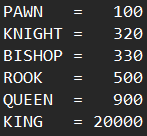
\includegraphics{figures/pieces_values.png}
        \caption{Base values for the pieces}
        \label{fig:piecesValues}
    \end{subfigure}
    \begin{subfigure}{0.49\textwidth}
        \centering
        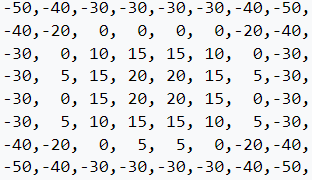
\includegraphics{figures/knight_value_table.png}
        \caption{Knight table}
        \label{fig:knightValueTable}
    \end{subfigure}
\end{figure}

\begin{figure}[h]
    \centering
    \caption{King tables}
    \begin{subfigure}{0.49\textwidth}
        \centering
        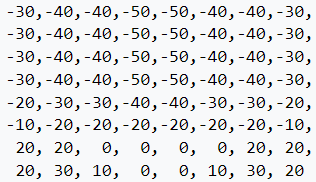
\includegraphics{figures/king_value_table_middlegame.png}
        \caption{King middlegame value table}
        \label{fig:kingValueTableMiddlegame}
    \end{subfigure}
    \begin{subfigure}{0.49\textwidth}
        \centering
        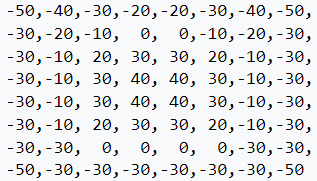
\includegraphics{figures/king_value_table_endgame.png}
        \caption{King endgame value table}
        \label{fig:kingValueTableEndgame}
    \end{subfigure}
\end{figure}

\subsection{Neural network}
\label{subsec:ch3sec3subsec2}

For the second evaluation function, I trained a neural network on master chess matches, which I will expand in a separate chapter.